\documentclass[a4paper,12pt]{article}
\usepackage{czech}
\usepackage[utf8]{inputenc}
\usepackage{a4wide}
\usepackage[dvipdfm]{graphicx}
\usepackage{graphics}
\usepackage{indentfirst}
\usepackage{fancyhdr}
\usepackage{setspace}
\usepackage{amsmath}
\usepackage{amssymb}
\usepackage{epsfig}

%%\usepackage{nopageno}
%%\usepackage{txfonts}
\usepackage[usenames]{color}

\begin{document}
\section{Úkol}
\begin{enumerate}
    \item Cílem studované úlohy je seznámit posluchače s vlastnostmi spekter gama záření získaných polovodičovým spektrometrem.
    Měření se provádí na spektrometru KJF s GeLi detektorem o objemu aktivní oblasti 55 cm$^3$ (průměr čela detektoru je 70 mm). 
    Měření je prováděno se zářiči s jednoduchým spektrem gama záření: $^{137}$Cs (E = 661.55 keV), $^{60}$Co (E = 1173.27 keV) a 
    $^{24}$Na (E = 1368.63 a 2754.03 keV), které jsou současně používány ke kalibraci spektrometru. K nastavení geometrue zážič-detektor 
    se používá jednoduchý nosič zářičů umožňující volbu různé geometrie.
\end{enumerate}

\section{Teoretický úvod}
Gama záření je typ radiaktivního záření, které je tvořeno fotony o vysokých energiích. Je to jeden ze způsobý, kterým radiaktivní izotopy snižují svou energii. K jeho detekci se používají spektrometry např z polovodičů, ako při této úloze, kde toto záření vytrhává elektrony z mříže díky čemuž dochází ke změně el. proudu v měřícím obvodu. Mimo samotného chtěného efektu na detektoru se v naměřeném spektru projevuje spousta vedlejších efektů, které jsou podrobně pospány v \cite{text}.

\section{Měření}
\subsection{Kalibrace}
Nejprve jsem provedli kalibraci spektrometru za pomoci Ra, jehož spektrum je dobře známo.
Ke kalibraci jsme využili 8 bodů spektra. Chyba se v případě píků pohybovala okolo jednoho keV. 
V případě určování hran je však tato chyba až o řád vyšší.

\begin{figure}
\begin{center}
% GNUPLOT: LaTeX picture with Postscript
\begingroup
  \makeatletter
  \providecommand\color[2][]{%
    \GenericError{(gnuplot) \space\space\space\@spaces}{%
      Package color not loaded in conjunction with
      terminal option `colourtext'%
    }{See the gnuplot documentation for explanation.%
    }{Either use 'blacktext' in gnuplot or load the package
      color.sty in LaTeX.}%
    \renewcommand\color[2][]{}%
  }%
  \providecommand\includegraphics[2][]{%
    \GenericError{(gnuplot) \space\space\space\@spaces}{%
      Package graphicx or graphics not loaded%
    }{See the gnuplot documentation for explanation.%
    }{The gnuplot epslatex terminal needs graphicx.sty or graphics.sty.}%
    \renewcommand\includegraphics[2][]{}%
  }%
  \providecommand\rotatebox[2]{#2}%
  \@ifundefined{ifGPcolor}{%
    \newif\ifGPcolor
    \GPcolorfalse
  }{}%
  \@ifundefined{ifGPblacktext}{%
    \newif\ifGPblacktext
    \GPblacktexttrue
  }{}%
  % define a \g@addto@macro without @ in the name:
  \let\gplgaddtomacro\g@addto@macro
  % define empty templates for all commands taking text:
  \gdef\gplbacktext{}%
  \gdef\gplfronttext{}%
  \makeatother
  \ifGPblacktext
    % no textcolor at all
    \def\colorrgb#1{}%
    \def\colorgray#1{}%
  \else
    % gray or color?
    \ifGPcolor
      \def\colorrgb#1{\color[rgb]{#1}}%
      \def\colorgray#1{\color[gray]{#1}}%
      \expandafter\def\csname LTw\endcsname{\color{white}}%
      \expandafter\def\csname LTb\endcsname{\color{black}}%
      \expandafter\def\csname LTa\endcsname{\color{black}}%
      \expandafter\def\csname LT0\endcsname{\color[rgb]{1,0,0}}%
      \expandafter\def\csname LT1\endcsname{\color[rgb]{0,1,0}}%
      \expandafter\def\csname LT2\endcsname{\color[rgb]{0,0,1}}%
      \expandafter\def\csname LT3\endcsname{\color[rgb]{1,0,1}}%
      \expandafter\def\csname LT4\endcsname{\color[rgb]{0,1,1}}%
      \expandafter\def\csname LT5\endcsname{\color[rgb]{1,1,0}}%
      \expandafter\def\csname LT6\endcsname{\color[rgb]{0,0,0}}%
      \expandafter\def\csname LT7\endcsname{\color[rgb]{1,0.3,0}}%
      \expandafter\def\csname LT8\endcsname{\color[rgb]{0.5,0.5,0.5}}%
    \else
      % gray
      \def\colorrgb#1{\color{black}}%
      \def\colorgray#1{\color[gray]{#1}}%
      \expandafter\def\csname LTw\endcsname{\color{white}}%
      \expandafter\def\csname LTb\endcsname{\color{black}}%
      \expandafter\def\csname LTa\endcsname{\color{black}}%
      \expandafter\def\csname LT0\endcsname{\color{black}}%
      \expandafter\def\csname LT1\endcsname{\color{black}}%
      \expandafter\def\csname LT2\endcsname{\color{black}}%
      \expandafter\def\csname LT3\endcsname{\color{black}}%
      \expandafter\def\csname LT4\endcsname{\color{black}}%
      \expandafter\def\csname LT5\endcsname{\color{black}}%
      \expandafter\def\csname LT6\endcsname{\color{black}}%
      \expandafter\def\csname LT7\endcsname{\color{black}}%
      \expandafter\def\csname LT8\endcsname{\color{black}}%
    \fi
  \fi
  \setlength{\unitlength}{0.0500bp}%
  \begin{picture}(7200.00,5040.00)%
    \gplgaddtomacro\gplbacktext{%
      \csname LTb\endcsname%
      \put(1474,704){\makebox(0,0)[r]{\strut{} 1}}%
      \put(1474,1518){\makebox(0,0)[r]{\strut{} 10}}%
      \put(1474,2332){\makebox(0,0)[r]{\strut{} 100}}%
      \put(1474,3147){\makebox(0,0)[r]{\strut{} 1000}}%
      \put(1474,3961){\makebox(0,0)[r]{\strut{} 10000}}%
      \put(1474,4775){\makebox(0,0)[r]{\strut{} 100000}}%
      \put(1778,484){\makebox(0,0){\strut{} 195}}%
      \put(2296,484){\makebox(0,0){\strut{}}}%
      \put(2332,484){\makebox(0,0){\strut{} 500}}%
      \put(2426,484){\makebox(0,0){\strut{}}}%
      \put(2622,484){\makebox(0,0){\strut{}Cs}}%
      \put(3239,484){\makebox(0,0){\strut{} 1000}}%
      \put(4147,484){\makebox(0,0){\strut{} 1500}}%
      \put(5054,484){\makebox(0,0){\strut{} 2000}}%
      \put(5962,484){\makebox(0,0){\strut{} 2500}}%
      \put(308,2739){\rotatebox{-270}{\makebox(0,0){\strut{}N}}}%
      \put(4237,154){\makebox(0,0){\strut{}$E$/keV}}%
      \put(1706,3716){\makebox(0,0)[l]{\strut{}hz}}%
      \put(2241,3392){\makebox(0,0)[l]{\strut{}h1}}%
      \put(2405,2902){\makebox(0,0)[l]{\strut{}h2}}%
    }%
    \gplgaddtomacro\gplfronttext{%
    }%
    \gplbacktext
    \put(0,0){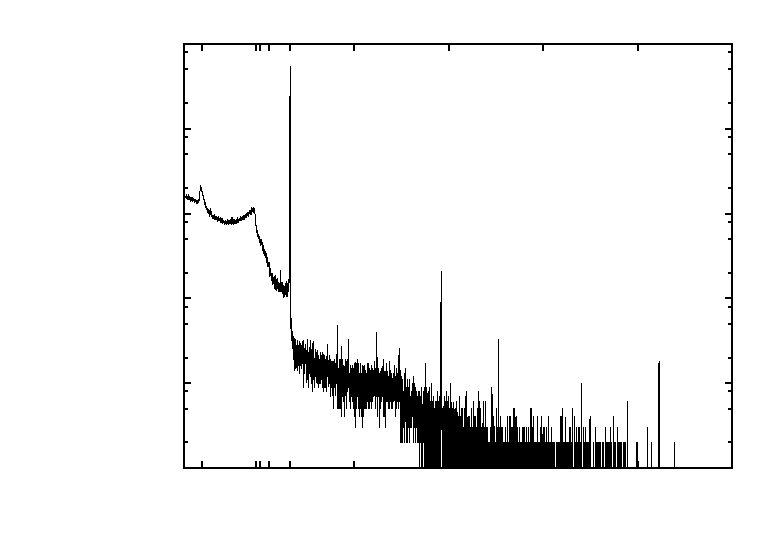
\includegraphics{spect1}}%
    \gplfronttext
  \end{picture}%
\endgroup

\end{center}
\caption{Naměřené spektrum Cs izotopu 137.}
\label{spect1}
\end{figure}

\subsection{Cs}
Dále jsme na spektrometr umístili Cs izotop 137 a pozorovali vzniklé spektrum, které je vidět na obrázku \ref{spect1}. 
Na tomto spektru je vidět jediný dominantní pík, který odpovídá energii gama zážení Cs. Odpovídá energii
\begin{eqnarray}
E=661.66 \mbox{keV},
\end{eqnarray}
což zcela přesně koresponduje teoretické hodnotě.
\begin{eqnarray}
E_{Na}=661.66\mbox{keV}
\end{eqnarray}

Dále můžeme na spektru pozorovat projevy Comptnova rozptylu. Comptnovy hrany se nachází na energiích
\begin{eqnarray}
E_{h1}=480 \mbox{keV} \\
E_{h2}=552 \mbox{keV}
\end{eqnarray}
Hrana zpětného odrazu je na energii
\begin{eqnarray}
E_{hz}=195 \mbox{keV}
\end{eqnarray}
Dle teorie by hodnoty těchto hran měli být
\begin{eqnarray}
E_{th1}=477.33 \mbox{keV} \\
E_{th2}=554.58 \mbox{keV}
\end{eqnarray}

\begin{figure}
\begin{center}
% GNUPLOT: LaTeX picture with Postscript
\begingroup
  \makeatletter
  \providecommand\color[2][]{%
    \GenericError{(gnuplot) \space\space\space\@spaces}{%
      Package color not loaded in conjunction with
      terminal option `colourtext'%
    }{See the gnuplot documentation for explanation.%
    }{Either use 'blacktext' in gnuplot or load the package
      color.sty in LaTeX.}%
    \renewcommand\color[2][]{}%
  }%
  \providecommand\includegraphics[2][]{%
    \GenericError{(gnuplot) \space\space\space\@spaces}{%
      Package graphicx or graphics not loaded%
    }{See the gnuplot documentation for explanation.%
    }{The gnuplot epslatex terminal needs graphicx.sty or graphics.sty.}%
    \renewcommand\includegraphics[2][]{}%
  }%
  \providecommand\rotatebox[2]{#2}%
  \@ifundefined{ifGPcolor}{%
    \newif\ifGPcolor
    \GPcolorfalse
  }{}%
  \@ifundefined{ifGPblacktext}{%
    \newif\ifGPblacktext
    \GPblacktexttrue
  }{}%
  % define a \g@addto@macro without @ in the name:
  \let\gplgaddtomacro\g@addto@macro
  % define empty templates for all commands taking text:
  \gdef\gplbacktext{}%
  \gdef\gplfronttext{}%
  \makeatother
  \ifGPblacktext
    % no textcolor at all
    \def\colorrgb#1{}%
    \def\colorgray#1{}%
  \else
    % gray or color?
    \ifGPcolor
      \def\colorrgb#1{\color[rgb]{#1}}%
      \def\colorgray#1{\color[gray]{#1}}%
      \expandafter\def\csname LTw\endcsname{\color{white}}%
      \expandafter\def\csname LTb\endcsname{\color{black}}%
      \expandafter\def\csname LTa\endcsname{\color{black}}%
      \expandafter\def\csname LT0\endcsname{\color[rgb]{1,0,0}}%
      \expandafter\def\csname LT1\endcsname{\color[rgb]{0,1,0}}%
      \expandafter\def\csname LT2\endcsname{\color[rgb]{0,0,1}}%
      \expandafter\def\csname LT3\endcsname{\color[rgb]{1,0,1}}%
      \expandafter\def\csname LT4\endcsname{\color[rgb]{0,1,1}}%
      \expandafter\def\csname LT5\endcsname{\color[rgb]{1,1,0}}%
      \expandafter\def\csname LT6\endcsname{\color[rgb]{0,0,0}}%
      \expandafter\def\csname LT7\endcsname{\color[rgb]{1,0.3,0}}%
      \expandafter\def\csname LT8\endcsname{\color[rgb]{0.5,0.5,0.5}}%
    \else
      % gray
      \def\colorrgb#1{\color{black}}%
      \def\colorgray#1{\color[gray]{#1}}%
      \expandafter\def\csname LTw\endcsname{\color{white}}%
      \expandafter\def\csname LTb\endcsname{\color{black}}%
      \expandafter\def\csname LTa\endcsname{\color{black}}%
      \expandafter\def\csname LT0\endcsname{\color{black}}%
      \expandafter\def\csname LT1\endcsname{\color{black}}%
      \expandafter\def\csname LT2\endcsname{\color{black}}%
      \expandafter\def\csname LT3\endcsname{\color{black}}%
      \expandafter\def\csname LT4\endcsname{\color{black}}%
      \expandafter\def\csname LT5\endcsname{\color{black}}%
      \expandafter\def\csname LT6\endcsname{\color{black}}%
      \expandafter\def\csname LT7\endcsname{\color{black}}%
      \expandafter\def\csname LT8\endcsname{\color{black}}%
    \fi
  \fi
  \setlength{\unitlength}{0.0500bp}%
  \begin{picture}(7200.00,5040.00)%
    \gplgaddtomacro\gplbacktext{%
      \csname LTb\endcsname%
      \put(1342,704){\makebox(0,0)[r]{\strut{} 1}}%
      \put(1342,1722){\makebox(0,0)[r]{\strut{} 10}}%
      \put(1342,2740){\makebox(0,0)[r]{\strut{} 100}}%
      \put(1342,3757){\makebox(0,0)[r]{\strut{} 1000}}%
      \put(1342,4775){\makebox(0,0)[r]{\strut{} 10000}}%
      \put(2064,484){\makebox(0,0){\strut{}J}}%
      \put(2239,484){\makebox(0,0){\strut{}}}%
      \put(2882,484){\makebox(0,0){\strut{}}}%
      \put(3834,484){\makebox(0,0){\strut{}Na$^2$}}%
      \put(4344,484){\makebox(0,0){\strut{}}}%
      \put(4510,484){\makebox(0,0){\strut{}}}%
      \put(5320,484){\makebox(0,0){\strut{}Cl}}%
      \put(5460,484){\makebox(0,0){\strut{}}}%
      \put(6411,484){\makebox(0,0){\strut{}Na}}%
      \put(308,2739){\rotatebox{-270}{\makebox(0,0){\strut{}N}}}%
      \put(4171,154){\makebox(0,0){\strut{}$E$/keV}}%
      \put(2125,3451){\makebox(0,0)[l]{\strut{}anti}}%
      \put(2869,2433){\makebox(0,0)[l]{\strut{}Na$^2_{SEP}$}}%
      \put(4265,1722){\makebox(0,0)[l]{\strut{}Cl$_{SEP}$}}%
      \put(4451,2028){\makebox(0,0)[l]{\strut{}Na$_{DEP}$}}%
      \put(5381,1722){\makebox(0,0)[l]{\strut{}Na$_{SEP}$}}%
    }%
    \gplgaddtomacro\gplfronttext{%
    }%
    \gplbacktext
    \put(0,0){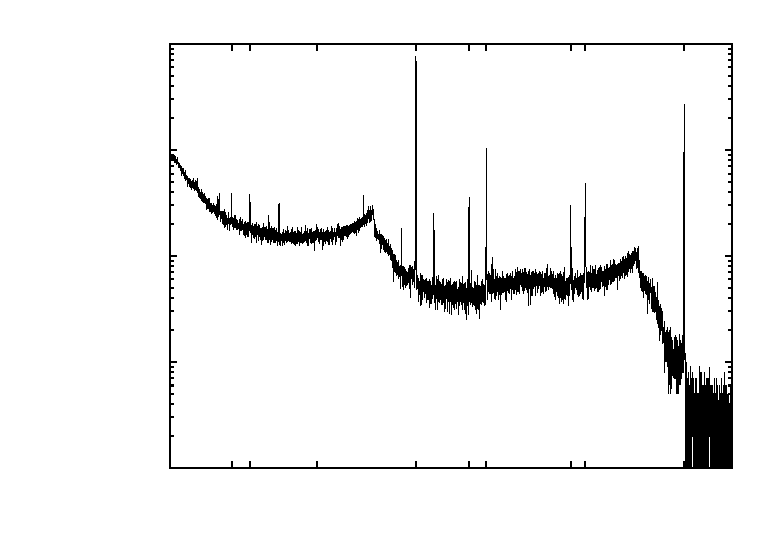
\includegraphics{spect2}}%
    \gplfronttext
  \end{picture}%
\endgroup

\end{center}
\caption{Naměřené spektrum radioaktivní soli.}
\label{spect2}
\end{figure}

\subsection{sůl}
Dále jsme pozorovali sůl ozařovanou neutronovým zářením. Tak v ní vznikly izotopy $^{24}$Na a radioaktivní izotop Cl.
Tam se mimo Comptnova rozpztylu navíc projevil efekt, při kterém z dvojice fotnů vzniká pár elektron, pozitron. Píky tohoto 
efektu jsou vyznačeny spolu s dalšímy body na obrázku \ref{spect2}. Jejich energetické hodnoty jsou
\begin{eqnarray}
E_{Na}=2753.82 \mbox{keV} \\
E_{NaSEP}=2242.77 \mbox{keV} \\
E_{NaDEP}=1731.84 \mbox{keV} \\
E_{Cl}=2167.28 \mbox{keV} \\
E_{ClSEP}=1642.51 \mbox{keV} \\
E_{Na2}=1368.50 \mbox{keV} \\
E_{Na2SEP}=856.83 \mbox{keV} \\
E_{ani}=510.95 \mbox{keV} \\
E_{J}=416.88 \mbox{keV}
\end{eqnarray}
Pro srovnání jsou teoretické energie 
\begin{eqnarray}
E_{tNa}=2754.03  \mbox{keV} \\
E_{tNaSEP}=2243.03 \mbox{keV} \\
E_{tNaDEP}=1732.03 \mbox{keV} \\
E_{tNa2}=1368.23  \mbox{keV} \\
E_{tNa2SEP}=857.23  \mbox{keV} \\
E_{tani}=511  \mbox{keV}
\end{eqnarray}
Pro úplnost jsem určil i hodnoty comptnových hran
\begin{eqnarray}
E_{hNa}=2521 \mbox{keV} \\
E_{h2Na}=2631 \mbox{keV} \\
E_{hNa2}=1157 \mbox{keV} \\
E_{h2Na2}=1253 \mbox{keV}
\end{eqnarray}
Pro srovnání opět uvádím teoretické hodnoty
\begin{eqnarray}
E_{thNa}=2520.22 \mbox{keV} \\
E_{th2Na}=2631.94 \mbox{keV} \\
E_{thNa2}=1152.93 \mbox{keV} \\
E_{th2Na2}=1251.39 \mbox{keV}
\end{eqnarray}

\section{Diksuze}
Na naměřených spektrech byli velmii dobře pozorovatelné všechny očekávané ekekty. Teoretické a tabulkové hodnoty se přesně  shodovali s naměřenými hodnotami dokonce s výrazně nižší chybou, než byla chyba fitu. Vliv pozadí byl řádově nižší než použité zářiče, takže neměli přílišný vliv na výsledky a proto ve spektrech nejsou žádné výrazné nadbytečné píky.

\section{Závěr}
Vyšetřil jsem spektra dvou různých zářičů, která jsou na obrázcích \ref{spect1} s \ref{spect2}, na kterých jsou také vyznačeny všechny významné body.

\begin{thebibliography}{5}
	\bibitem{text} \textbf{Studijní text na praktikum IV} \\http://physics.mff.cuni.cz/vyuka/zfp/txt\_400.pdf (9. 10. 2012)
    \bibitem{chyba} \emph{J. Englich}: \textbf{Zpracování výsldků fyzikálních měření} \\ LS 1999/2000
\end{thebibliography}
\end{document}
